\documentclass[../main.tex]{subfiles}
\graphicspath{{\subfix{../images/}}}
\begin{document}
\chapitre{Annexes}

\begin{figure}[h]
  \centering
  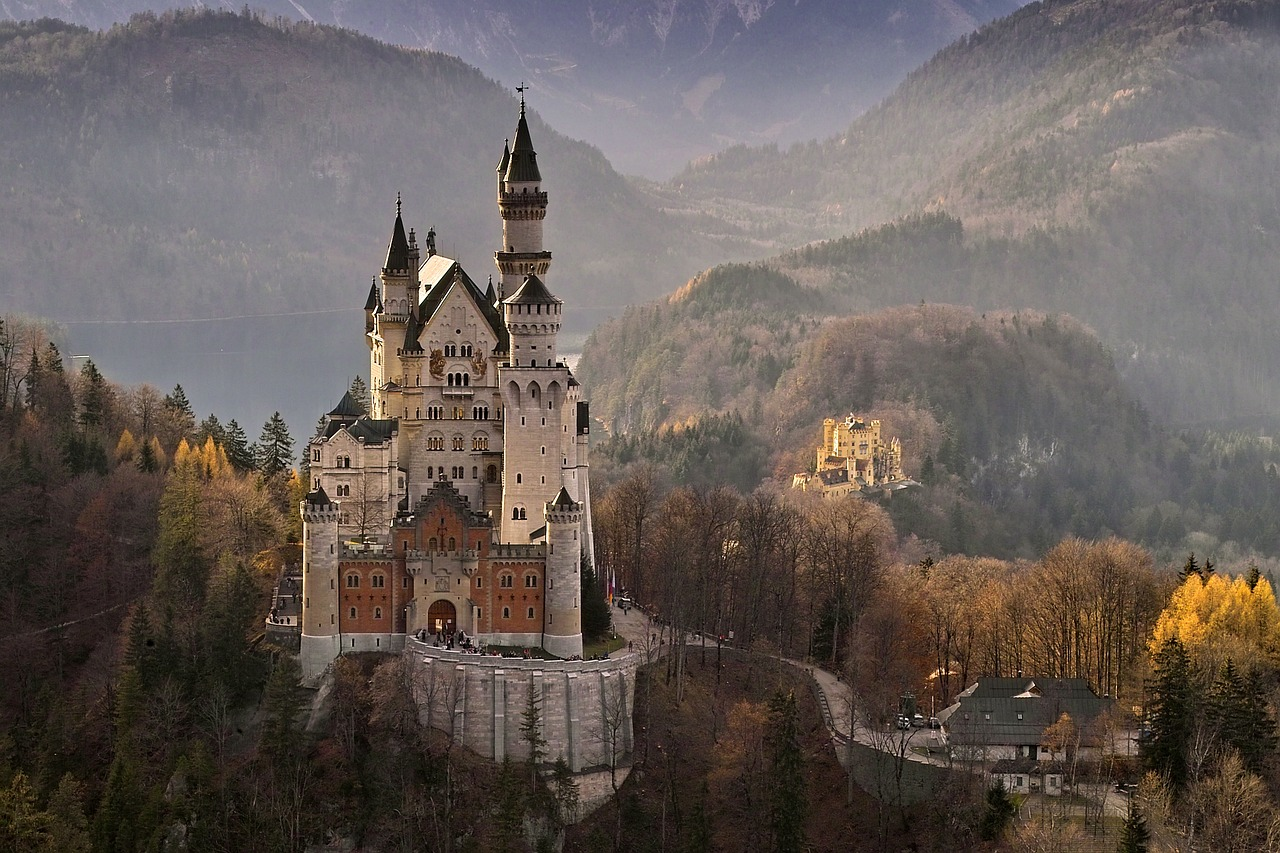
\includegraphics[width=\textwidth,height=0.4\textheight,keepaspectratio]{images/photos/batiment}
  \captionsetup{font=small,labelfont=bf, justification=centering}
  \caption{Futur nouveau bâtiment de The Pokémon Entreprise}
  \label{fig:batiment}
\end{figure}

\begin{figure}[h]
  \centering
  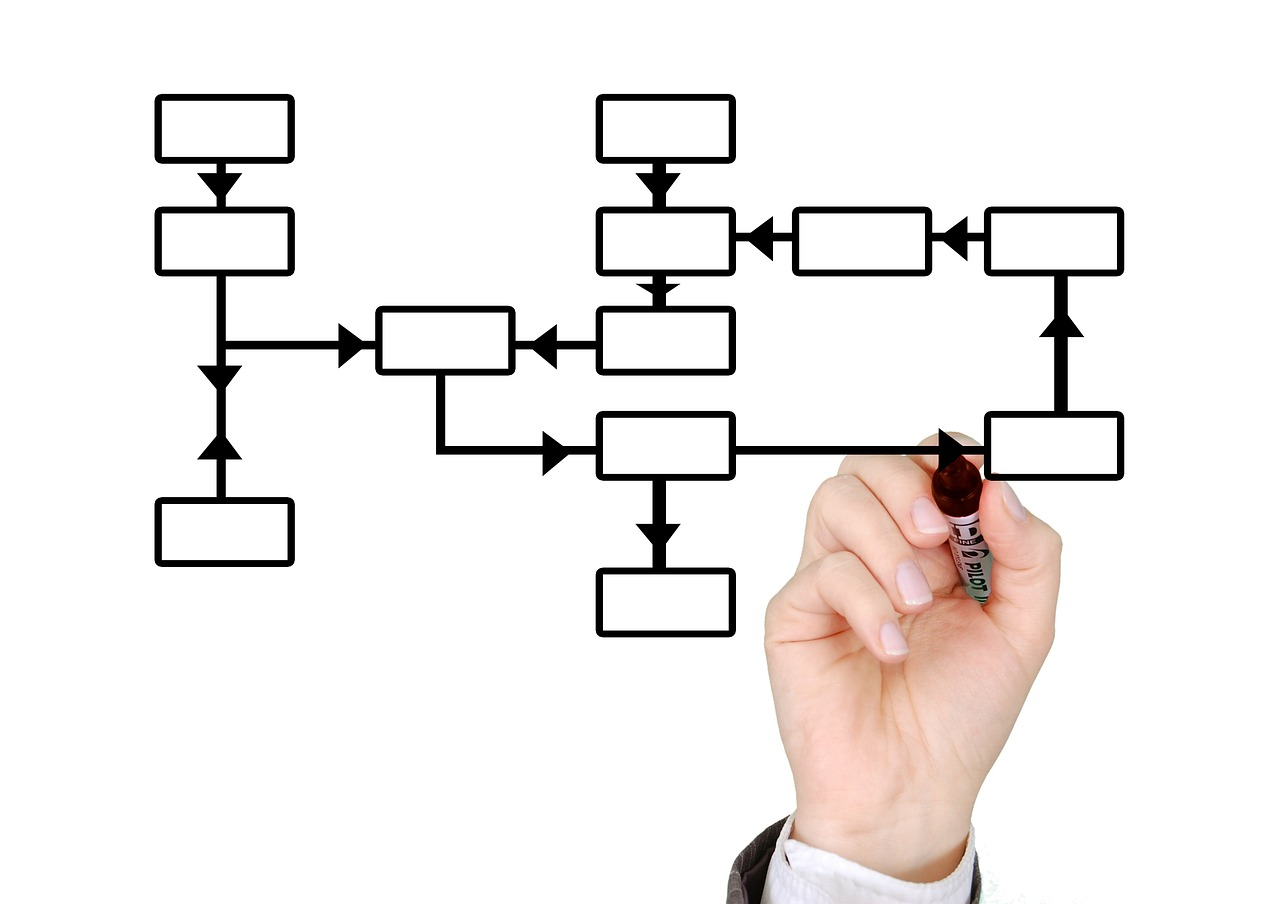
\includegraphics[width=\textwidth,height=0.4\textheight,keepaspectratio]{images/organigrammes/organigramme}
  \captionsetup{font=small,labelfont=bf, justification=centering}
  \caption{L'organigramme de The Pokémon Entreprise}
  \label{fig:organigramme}
\end{figure}

\begin{figure}[h]
  \centering
  
\includegraphics[width=\textwidth,height=0.4\textheight,keepaspectratio]{images/pokemons/pikachu_gros}
  \captionsetup{font=small,labelfont=bf, justification=centering}
  \caption{Un dessin de Pikachu en surpoids}
  \label{fig:pikachu_gros}
\end{figure}

\begin{figure}[h]
  \centering
  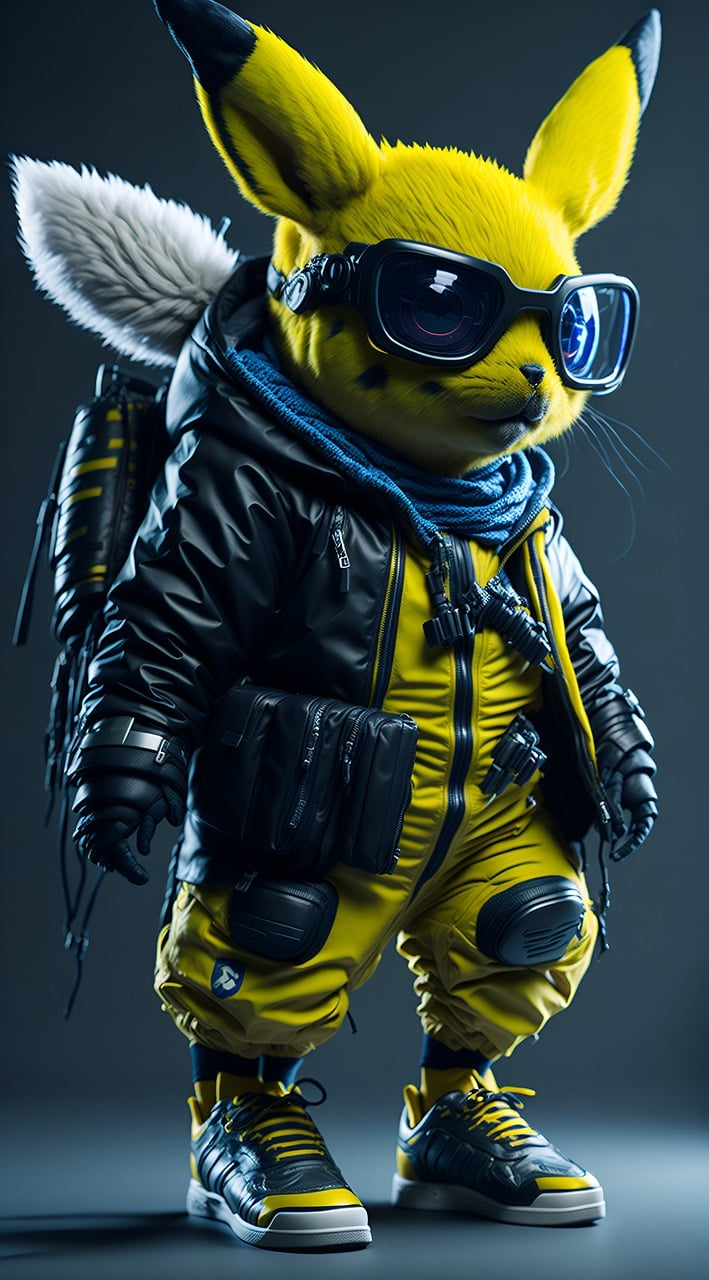
\includegraphics[width=\textwidth,height=0.4\textheight,keepaspectratio]{images/pokemons/pikachu_style}
  \captionsetup{font=small,labelfont=bf, justification=centering}
  \caption{Pikachu parti en mission et portant des lunettes}
  \label{fig:pikachu_style}
\end{figure}

\end{document}